\section{Direkt GPIO}
\begin{frame}{Direkter Zugriff auf die \hw}
 \begin{itemize}
  \item die Register
  \item als Memory
  \item Siehe \cod{src/gpio.h}
 \end{itemize}
\end{frame}

\begin{frame}{Informationen}
 \begin{itemize}
  \item \cod{cat /proc/iomem}
 \end{itemize}
\end{frame}


\begin{frame}{Register}{im Memory}
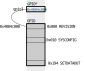
\includegraphics[height=0.75\textheight]{hw-gpio.pdf}
\begin{textblock}{100}(70,60)
\begin{itemize}
 \item \cod{GPIO* \_\_iomem  gpio1=???}
 \item \cod{gpio1=ioremap(0x4804c000,0x1000)}
\end{itemize}
\end{textblock}
\end{frame}

\begin{frame}{Die einzelnen Bits}{die Operationen}
 \begin{description}
  \item[setBit] Operation $|$
  \item[clrBit] Operation $\&$
 \end{description}
\end{frame}

\begin{frame}{Loadable Kernel Module (LKM)}{\cod{gpio-1.c}}
\begin{itemize}
 \item Manual \cod{spruh73l.pdf} Abschnitt 25
 \item \cod{gpio.h} die einzelnen Register:
 \begin{description}[CLEARDATAOUT]
  \item[REVSION] f�r Test
  \item[OE] OutputEnable
  \item[DATAIN] Data In
  \item[CLEARDATAOUT] L�scht Bit
  \item[SETDATAOUT] Setzt Bit
 \end{description}
 \item \href{https://elixir.bootlin.com/linux/latest/source/arch/alpha/include/asm/io.h\#L286}
            {\cod{ioremap}}
 \item \href{https://elixir.bootlin.com/linux/latest/source/arch/alpha/include/asm/io.h\#L306}
            {\cod{iounmap}}
\end{itemize}
\end{frame}
